\title{Computer Networks - CS 204} % You may change the title if you want.

\author{Rishit Saiya - 180010027, Summary}

\date{\today}

\documentclass[12pt]{article}
\usepackage{fullpage}
\usepackage{enumitem}
\usepackage{amsmath,mathtools}
\usepackage{amssymb}
\usepackage[super]{nth}
\usepackage{textcomp}
\usepackage{hyperref}
\begin{document}
\maketitle

\section{Data Link Layer}
This layer of OSI model is responsible for the transfer of information, framing and error checking.

This layer is further divided into two sub layers as follows:
    \begin{itemize}
        \item Logical Link Control Layer (LLC)
        \item Medium Access Control Layer (MAC)
    \end{itemize}

The main motivation behind introducing this layer was for the following issues:
\begin{itemize}
    \item \textbf{\textit{Sharing Wire}} \\
    One of the huge constraints arising due to the physical layer. It also includes the problems of Multiple hosts, wires for everybody in the network, sharing the same wire among the systems in the network.
    \item \textbf{\textit{Listen and Speak}} \\
    These include cases like only one speakers, multiple speaker, etc.
    \item \textbf{\textit{The Recipient Anonymity}} \\
    Here the constraints include the address, addressing format and after that where the link has to send with the data. Hence we don't know who is the receipent only with the address. To suffice the additional information, we have include parameters in the Data Link Layers.
\end{itemize}

\section{Medium Access Control Layer (MAC)}
The layer below Logical Link Control Layer, which provides logic for gaining access to the network is the MAC Layer.

This sublayer is primarily used in broadcast or shared channel networks. MAC protocols enables 2 stations using shared communication resource to establish, maintain or terminate a connection. \\
For example: Satellite, Cellular, Ethernet, etc.

In compliance with the IEEE 802 standards, the functions of the MAC layers are as follows:
\begin{itemize}
    \item Data Assembly $\And$ dismantle into frames.
    \item Govern access to LAN transmission medium.
\end{itemize}

%---------------------------------------------------------------------

\section{Logical Link Control Layer (LLC)}
The sublayer which is responsible for transmission of link level Protocol Data Unit (PDU) between intermediate switching mode is the Logic Link Control Layer.

The characteristics of this layer are as follows: 
\begin{itemize}
    \item It must support multi-access shared medium nature of link.
    \item It is relieved from the details of link access by MAC Layer.
\end{itemize}

In compliance with the IEEE 802 standards, the functions of the LLC layers are as follows:
\begin{itemize}
    \item Flow and Error Control.
    \item Interface to a higher level.
\end{itemize}

%---------------------------------------------------------------------

\section{MAC Generic Frame Format}

\begin{figure}
    \centering
    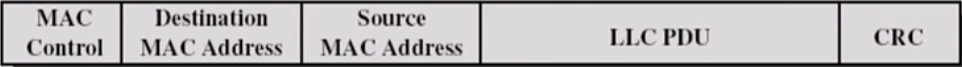
\includegraphics[width=15cm, height=1cm]{mac_frame.png}
    \caption{MAC Generic Frame Format}
\end{figure}

The MAC Generic Frame format is as shown in the Figure 1. The details for the same are as follows:

\begin{itemize}
    \item \textbf{\textit{MAC Control}} \\
        It contains control information for the functioning of the MAC protocol. \\
        For example: Priority Level
    \item \textbf{\textit{Destination MAC Address}} \\
        The destination physical attachment point on the LAN for this frame.
    \item \textbf{\textit{Source MAC Address}} \\
        The source physical attachment point on the LAN for this frame.
    \item \textbf{\textit{LLC PDU}} \\
        The LLC data from the next higher layer.
    \item \textbf{\textit{CRC}} \\
        The Cyclic Redundancy Check (CRC) field is used to check if a transmission error has occurred.
\end{itemize}

%---------------------------------------------------------------------

\section{MAC Techniques}
We know that when an internet packet has to hop from source to destination, it has to logically resolve IP addresses to MAC address at every hop and then consecutively push to the next MAC address manifesting to the next IP address and so on. For this resolution Address Resolution Protocol (ARP) is used. The MAC techniques involved are:
\begin{enumerate}[label=(\alph*)]
    \item \textbf{\textit{Synchronous Technique}} \\
    The characteristics of Synchronous Technique are as follows:
        \begin{itemize}
            \item A specific capacity is dedicated to a connection.
            \item The approach is similar as in circuit-switching FDM or TDM, so not optimal for LANs/MANs. It is because, in metropolitan cities, the connectivity is so unpredictable as there lot of users.
        \end{itemize}
    \item \textbf{\textit{Asynchronous Technique}} \\
    The characteristics of Asynchronous Technique are as follows:
        \begin{itemize}
            \item The capacity is allocated in a dynamic fashion. It is dependent in response to demand.
            \item Asynchronous Technique is further divided into 3 categories:
                \begin{enumerate}
                    \item Contention
                    \item Reservation
                    \item Round Robin
                \end{enumerate}
        \end{itemize}
    
    \textbf{\textit{Contention Technique}} \\
    It is very simple to implement and efficient for light loads. There is no control exercised to determine who is the next recipient. For heavy traffic, the mode of technique shifts where the concentration is on short, sporadic transmissions such as interactive terminal-host traffic.
    
    \textbf{\textit{Reservation Technique}} \\
    It is used for stream traffic which is comprised of voice, bulk file transfer, etc. It is useful for network device wishing to transmit reserve slots for an extended period. It is to be noted that in this technique, the time on the medium is divided into slots, like synchronous TDM.
    
    \textbf{\textit{Round Robin Technique}} \\
    It is an efficient technique when many stations have data to transmit over an extended period of time. Here each station in turn is granted the right to transmit. After each station finishes transmitting, it passes the right to transmit to the next station in the logical sequence.
    
\end{enumerate}

%-----------------------------------------------------------------------

\section{CSMA/CD and Token Passing}
With the reference of above mentioned motivations to develop Data Link Layer, the methods used in Media Access Control Layer are: 
\begin{itemize}
    \item Carrier Sense Multiple Access with Collision Detection for \textit{bus topologies}.
    \item Control Token or Token Passing for \textit{bus and ring topologies}.
\end{itemize}

\subsection{CSMA/CD}
Before explaining CSMA/CD, we must understand about Bus Topology. \\
\textbf{\textit{Bus Topology:}} \\
A number of nodes share a common communication channel (wire) is known as Bus Topology. It is depicted in Figure 2.

\begin{figure}
    \centering
    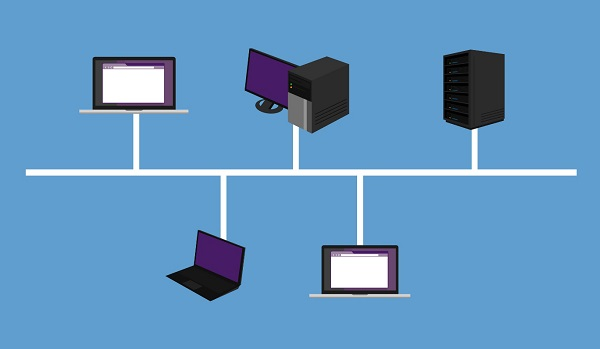
\includegraphics[width=10cm, height=5cm]{bus.png}
    \caption{Bus Topology}
\end{figure}

CSMA/CD is used in bus type network topologies. It is also used in the traditional Ethernet also.

The working of CSMA/CD is as follows:
\begin{enumerate}[label=(\alph*)]
    \item The \textbf{\textit{Source Station}}, where the transmission occurs, assembles a packet comprising of the destination address, the data and control information.
    \item The source station listens to the cable to determine if the bus is currently in use. \\
    If yes, it waits until the bus is free, else, it transmits the packet. This process is known as \textbf{\textit{Carrier Sensing}}.
    \item During transmission, the source station continues to listen to the cable to detect if another station has also initiated a transmissions this causing a \textbf{\textit{Collision}}. This process is known as \textbf{\textit{Collision Detection}}.
    \item If a collision is detected then, to ensure all the stations are aware of the collision, the source station transmits a random bit pattern known as the \textbf{\textit{Jam Sequence}}.
    \item Stations involved in a collision then back off for a random period before retrying for a packet transmission.
\end{enumerate}

For a perfect idea, it is as depicted in Figure 3.

\begin{figure}
    \centering
    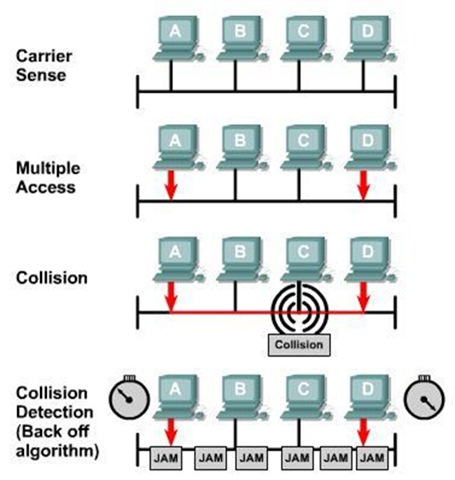
\includegraphics[width=10cm, height=10cm]{csma.png}
    \caption{CSMA/CD}
\end{figure}

For an algorithmic sense, it is given in Figure 4. It is self-explanatory. \\

\begin{figure}
    \centering
    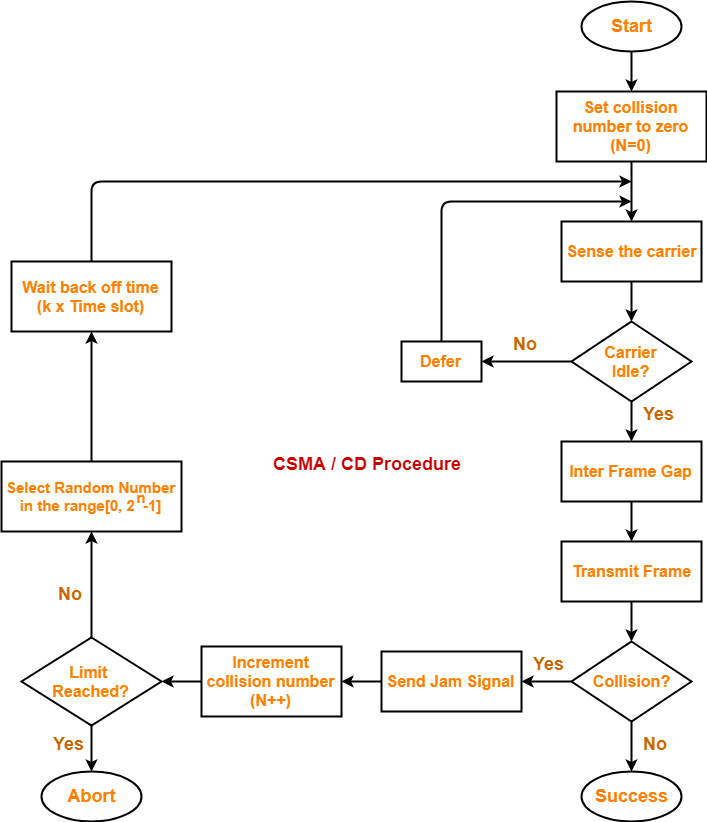
\includegraphics[width=10cm, height=10cm]{csma_algo.png}
    \caption{CSMA/CD Algorithm}
\end{figure}

\textbf{Note:} The worst case Collision Detection Time will be 2 $\times$ $T_{prop}$ (Propagation time from one host to another host in a network).

%---------------------------------------------------------------------

\subsection{Control Token or Token Passing}
The Control Token technique uses a control or a permission token to share the communication resource between a number of nodes. This technique is applicable to both bus and ring network topologies.

This token is passed from one station to another according to a defined set of rules. A station may transmit a frame only when it has possession of the token and after it has transmitted the frame, it passes the token on, to allow another station to access the transmission medium.

The working of CSMA/CD is as follows:
\begin{enumerate}[label=(\alph*)]
    \item Irrespective of using a ring or a bus network topology, a \textbf{\textit{Logical Ring}} is established which links all the nodes using the physical medium.
    \item A \textbf{\textit{Permission (Single Control Token)}} is initiated at one of the nodes.
    \item The token is passed from node to node around the logical ring until it arrives at a node waiting to send a frame which contains the information.
    \item The node captures the token and transmits the frame.
    \item When the transmission ends, the node releases the token to the next node in the logical ring.
\end{enumerate}

The Token Passing in Ring Network Topology is as depicted in Figure 5.
\begin{figure}
    \centering
    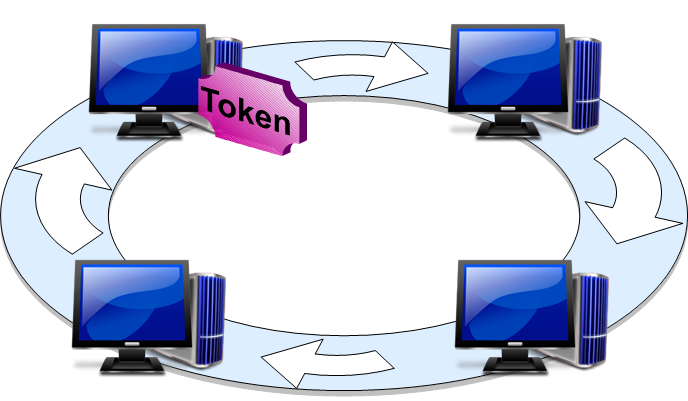
\includegraphics[width=10cm, height=5cm]{token_ring.png}
    \caption{Token Passing in Ring Network Topology}
\end{figure}

The Token Passing in Bus Network Topology is as depicted in Figure 6.
\begin{figure}
    \centering
    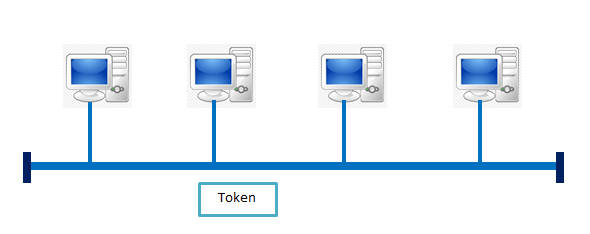
\includegraphics[width=10cm, height=5cm]{token_bus.png}
    \caption{Token Passing in Bus Network Topology}
\end{figure}

%---------------------------------------------------------------------

\section{Taxonomy of MAC Protocols}
With the motive of making protocols more efficient, fair and simple, decentralised (To avoid network failures), we have broadly divided our design fashion into 3 broad classes to suffice our motives. They are given as follows:

\begin{itemize}
    \item \textbf{\textit{Channel Partitioning}} \\
        Division of channel into smaller pieces of frequency in case of FMD or time in case of TMD and then the piece's allocation to the node for exclusive node is done here.
    \item \textbf{\textit{Random Access}} \\
        The recoveries from the collisions is done in this class.
    \item \textbf{\textit{Shared Access}} \\
        In this class, main motive is to be closely coordinated with shared accesses so as to avoid and minimize collisions.
\end{itemize}

\end{document}